\documentclass[fontset=mac]{ctexart}
\usepackage{amsmath}
\usepackage{amssymb}
\usepackage{geometry}
\usepackage{booktabs} %处理三线表
\geometry{a4paper,scale=0.8}
\usepackage{graphicx}
\usepackage{float}
\usepackage{algorithm}
\usepackage{algpseudocode}
\usepackage{amsmath}
\renewcommand{\algorithmicrequire}{\textbf{Input:}}  % Use Input in the format of Algorithm
\renewcommand{\algorithmicensure}{\textbf{Output:}} % Use Output in the format of Algorithm

\title{偏微分方程数值解大作业}
\author{于冰冰 21901037 数硕1903}
\date{\today}

\begin{document}
	\maketitle
	\tableofcontents
	\newpage
	\section{简介}
	微分方程指含有未知函数及其偏导数的方程,它描述了自变量、未知函数及其偏导数之间的关系。只有一个变量的情景是常微分方程,多个变量下是偏微分方程。如有两个独立变量时,二阶偏微分方程的一般形式是:
	$$
	a \frac{\partial ^2 \phi}{\partial x^2} + b \frac{\partial ^ 2 \phi}{\partial x \partial y} + c \frac{\partial ^ 2 \phi}{\partial y^2} + d \frac{\partial \phi}{\partial x} + e \frac{\partial \phi}{\partial y} + f \phi + g =0
	$$
	
	在上式中,我们假定了系数$a,b,c,d,e,f,g$不包含$\phi$ 及其高阶导数(否则方程就不是二阶的),这是线性的偏微分方程。否则就是非线性的偏微分方程。系数$a,b,c,d,e,f,g$可以是独立变量$x$和$y$的函数。在$a,b,c$不全为$0$的情况下,如果$b^2<4ac$,称为椭圆形偏微分方程,$b^2=4ac$是抛物线形,$b^2>4ac$是双曲线型。
	
	例如:二维的Poisson方程$$
	\frac{\partial^{2} \phi}{\partial x^{2}}+\frac{\partial^{2} \phi}{\partial y^{2}}=-\rho(x, y)
	$$
	是椭圆形,而波动方程
	$$
	\frac{\partial^{2} \phi}{\partial x^{2}}-\frac{1}{v^{2}} \frac{\partial^{2} \phi}{\partial t^{2}}=0
	$$
	是双曲线型,扩散方程
	$$
	\frac{\partial \phi}{\partial t}=\frac{\partial}{\partial x}\left(D \frac{\partial \phi}{\partial x}\right)+S(x, t)
	$$
	是抛物线形。下面将对三种形式的偏微分方程数值解法进行讨论和实验。
	
	\newpage
	\section{椭圆形偏微分方程求解}
	考虑如下带Dirichlet边界条件的Poisson方程:
	$$
	\left\{\begin{array}{l}
		-\Delta u=f \quad \text { in } \Omega \\
		u=\alpha \text { on } \partial \Omega
	\end{array}\right.
	$$
	式中$\Omega = (0,a) \times (0,b)$,$f$是定义在$\Omega$上某个函数,而$\alpha$是定义在$\Omega$边界$\partial \Omega$上的某一函数。
	先导出求解以上Poisson方程的五点差分格式,将区域$\Omega$在$x$方向和$y$方向分别进行$I+1$和$J+1$等分,则$x$方向和$y$方向的网格步长分别为:
	$$
	h=a /(I+1), \quad k=b /(J+1)
	$$
	目标点为$x_i=ih,y_j=jk,0<i<I+1,0<j<J+1$
	\begin{figure}[H]
		\centering
		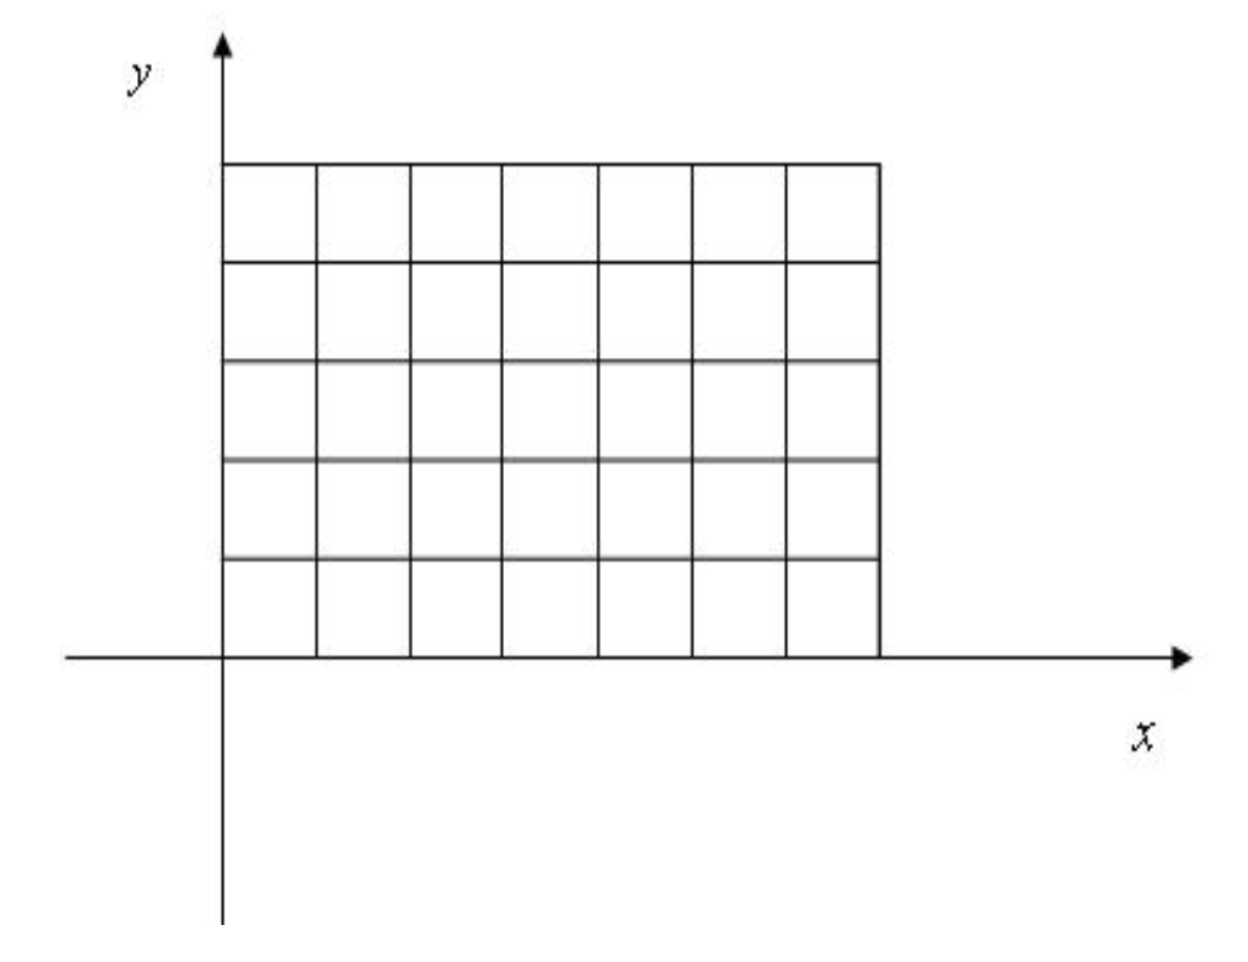
\includegraphics[width=0.7\linewidth]{fig/fig1}
		\caption{矩形网格区域划分}
	\end{figure}
	
	求解Poisson方程的五点差分格式如下:
	$$
	\left\{\begin{array}{l}
		-\Delta_{h} u_{i j}=f_{i j}, \quad\left(x_{i}, y_{j}\right) \in \Omega_{h} \\
		u_{i j}=\alpha_{i j}, \quad\left(x_{i}, y_{j}\right) \in \partial \Omega_{h}
	\end{array}\right.
	$$
	其中
	$$
	\Delta_{h} u_{i j}=\frac{u_{i+1, j}-2 u_{i j}+u_{i-1, j}}{h^{2}}+\frac{u_{i, j+1}-2 u_{i j}+u_{i, j-1}}{k^{2}}
	$$
	
	不失一般性,假设在单位正方形区域考虑,$a=b=1$。则求解它的五点差分格式可以写成如下矩阵方程:
	$$
	AU+UB=F
	$$
	其中
	$$
	\begin{aligned}
		&\boldsymbol{A}=\frac{1}{h^{2}}\left[\begin{array}{ccccc}
			2 & -1 & & & \\
			-1 & 2 & -1 & & \\
			& \ddots & \ddots & \ddots & \\
			& & -1 & 2 & -1 \\
			& & & -1 & 2
		\end{array}\right]_{I \times I}, \quad \boldsymbol{B}=\frac{1}{k^{2}}\left[\begin{array}{ccccc}
			2 & -1 & & & \\
			-1 & 2 & -1 & & \\
			& \ddots & \ddots & \ddots & \\
			& &  -1 & 2 & -1 \\
			& &  & -1 & 2 \\
		\end{array}\right]_{J \times J}\\ 
	\end{aligned}
	$$
		
		$$
		U=\left[\begin{array}{cccc}
			u_{11} & u_{12} & \cdots & u_{1, J} \\
			u_{21} & u_{22} & \cdots & u_{2, J} \\
			\cdots & \cdots & \cdots & \cdots \\
			u_{I 1} & u_{I 2} & \cdots & u_{I J}
		\end{array}\right],
		$$
		
		$$
		F=\left[\begin{array}{ccccc}
			f_{1,1}+\frac{1}{h^{2}} u_{0,1}+\frac{1}{k^{2}} u_{1,0} & f_{1,2}+\frac{1}{h^{2}} u_{0,2} & \cdots & f_{1, J-1}+\frac{1}{h^{2}} u_{0, J-1} & f_{1, J}+\frac{1}{h^{2}} u_{0, J}+\frac{1}{k^{2}} u_{1, J+1} \\
			f_{2,1}+\frac{1}{k^{2}} u_{2,0} & f_{2,2} & \cdots & f_{2, J-1} & f_{2, J}+\frac{1}{k^{2}} u_{2, J+1} \\
			\vdots & \ldots & \cdots & \cdots & \vdots \\
			f_{I-1,1}+\frac{1}{k^{2}} u_{I-1,0} & f_{I-1,2} & \cdots & f_{I-1, J-1} & f_{I-1, J}+\frac{1}{k^{2}} u_{I-1, J+1} \\
			f_{I, 1}+\frac{1}{h^{2}} u_{I+1,1}+\frac{1}{k^{2}} u_{I, 0} & f_{I, 2}+\frac{1}{h^{2}} u_{I+1,2} & \cdots & f_{I, J-1}+\frac{1}{h^{2}} u_{I+1,2} & f_{I, J}+\frac{1}{h^{2}} u_{I+1, J}+\frac{1}{k^{2}} u_{I, J+1}
		\end{array}\right]_{I \times J}
		$$
		
		$$
		=\left[f_{i, j}\right]_{I \times J}+\frac{1}{h^{2}}\left[\begin{array}{ccccc}
			u_{0,1} & u_{0,2} & \cdots & u_{0, J-1} & u_{0, J} \\
			0 & 0 & \cdots & 0 & 0 \\
			\vdots & \cdots & \cdots & \cdots & \vdots \\
			0 & 0 & \cdots & 0 & 0 \\
			u_{I+1,1} & u_{I+1,2} & \cdots & u_{I+1, J-1} & u_{I+1, J}
		\end{array}\right]_{I \times J} \quad+\frac{1}{k^{2}}\left[\begin{array}{ccccc}
			u_{1,0} & 0 & \cdots & 0 & u_{1, J+1} \\
			u_{2,0} & 0 & \cdots & 0 & u_{2, J+1} \\
			\vdots & \cdots & \cdots & \cdots & \vdots \\
			u_{I-1,0} & 0 & \cdots & 0 & u_{I-1, J+1} \\
			u_{I, 0} & 0 & \cdots & 0 & u_{I, J+1}
		\end{array}\right]_{I \times J}
		$$

	在进行数值实验时,我们选取
	$$
	u(x, y)=\sin (2 \pi n x)+\sin (2 \pi n y)+x^{2}
	$$
	那么
	$$
	-\Delta u(x, y)=4 n^{2} \pi^{2}[\sin (2 \pi n x)+\sin (2 \pi n y)]-2=f(x, y)
	$$
	其中$n$越大,原函数震荡的频率越高,对网格剖分的精细程度也就越高。函数的形状为:
	\begin{figure}[H]
		\centering
		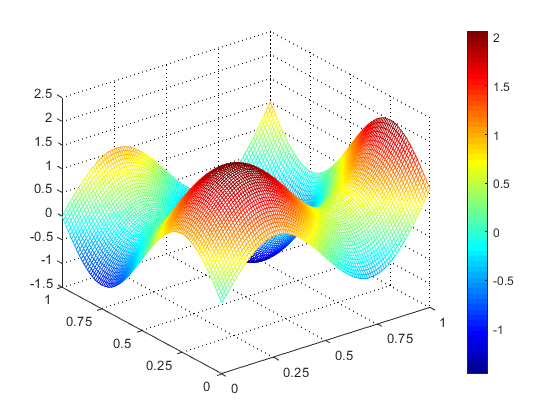
\includegraphics[width=0.7\linewidth]{fig/u}
		\caption{曲面 $u(x, y)=\sin (2 \pi n x)+\sin (2 \pi n y)+x^{2}, n=1$}
	\end{figure}
	
	
	\subsection{快速DST方法求解}
	记$\mathbf{P}=[sin(ij\pi h)] \in \mathbb{R}^{I \times I}$和$\mathbf{Q}=[sin(ij\pi k)] \in \mathbb{R}^{J \times J}$,求解五点差分格式的快速求解算法如下:
	
	\textbf{求解Poisson方程五点差分格式的快速DST算法}
	\begin{enumerate}
		\item[\textbf{步1.}] 给出划分数$I+1,J+1$,得步长$h = \frac{1}{I+1}, k = \frac{1}{J+1}$\\
		形成向量$\lambda$,其第$i$位置的元素$\lambda_i$为$\frac{4}{h^2} \sin^2 \frac{i \pi h}{2},1 \le i \le I$\\
		形成向量$\mu$,其第$j$位置的元素$\lambda_j$为$\frac{4}{k^2} \sin^2 \frac{j \pi k}{2},1 \le j \le J$\\
		计算矩阵$F$,其第$(i,j)$位置的元素为$f(ih,jk),1\le i \le I, 1 \le j \le J$
		\item[\textbf{步2.}] 使用快速DST计算矩阵$\mathbf{V} = \mathbf{PFQ}$
		\item[\textbf{步3.}] 计算矩阵$\mathbf{W} = [w_{ij}]$,
		$$
		w_{i j}=\frac{4 h k v_{i j}}{\lambda_{i}+\mu_{j}}
		$$
		\item[\textbf{步4.}] 使用快速DST计算矩阵$\mathbf{U} = \mathbf{PWQ}$
	\end{enumerate}
	数值结果如下:
	\begin{figure}[H]
		\centering
		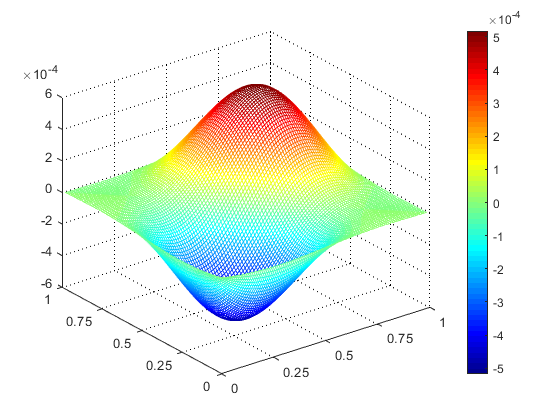
\includegraphics[width=0.7\linewidth]{fig/dst}
		\caption{快速DST算法,取N=100,n=1时的绝对误差曲面}
	\end{figure}
	可以看到对于该函数,绝对误差被控制在了$10^{-4}$量级,由于边界一定是精确解,在边界处误差为零,然后往中心区域误差逐渐累积,在内部达到峰值。

	\subsection{二维的紧致差分格式}
	对于五点差分格式,可以进行如下推广:不妨令$I=J=N$
	$$
	A U+U B=W F+F W+G
	$$
	其中
	$$
	A=\frac{1}{h^{2}}\left[\begin{array}{ccccc}
		2 & -1 & & & \\
		 -1 & 2 & -1 & & \\ 
		 & \ddots & \ddots & \ddots & \\ 
		 & & -1 & 2 & -1 \\
		  & & & -1 & 2\end{array}
	  \right]_{N \times N}, \quad, 
	  \quad B=\frac{1}{k^{2}}\left[\begin{array}{ccccc}
	  	2 & -1 & & & \\
	  	 -1 & 2 & -1 & & \\
	  	  & \ddots & \ddots & \ddots & \\
	  	   & & -1 & 2 & -1 \\ 
	  	   & & & -1 & 2
  	   \end{array}\right]_{N \times N}
	$$
	$$
	U=\left[\begin{array}{cccc}u_{1,1} & u_{1,2} & \cdots & u_{1, N} \\ u_{2,1} & u_{2,2} & \cdots & u_{2, N} \\ \cdots & \cdots & \cdots & \cdots \\ u_{N, 1} & u_{N, 2} & \cdots & u_{N, N}\end{array}\right]_{N \times N}, \quad F=\left[\begin{array}{ccccc}f_{1,1} & f_{1,2} & \cdots & f_{1, N} \\ f_{2,1} & f_{2,2} & \cdots & f_{2, N} \\ \cdots & \cdots & \cdots & \cdots \\ f_{N, 1} & f_{N, 2} & \cdots & f_{N, N}\end{array}\right]_{N \times N}
	$$
	$$
	W=\frac{1}{12}\left[\begin{array}{ccccc}4 & 1 & & & \\ 1 & 4 & 1 & & \\ & \ddots & \ddots & \ddots & \\ & & 1 & 4 & 1 \\ & & & 1 & 4\end{array}\right]_{N \times N}
	$$
	$$
	\begin{aligned}
		G = 
		\left[\begin{array}{ccccc}
			\frac{1}{12} f_{0,1}+\frac{1}{h^{2}} u_{0,1} & \frac{1}{12} f_{0,2}+\frac{1}{h^{2}} u_{0,2} & \cdots & \frac{1}{12} f_{0, N-1}+\frac{1}{h^{2}} u_{0, N-1} & \frac{1}{12} f_{0, N}+\frac{1}{h^{2}} u_{0, N} \\
			0 & 0 & \cdots & 0 & 0 \\
			\vdots & \cdots & \cdots & \cdots & 0 \\
			0 & 0 & \cdots & 0 & 0 \\
			\frac{1}{12} f_{N+1,1}+\frac{1}{h^{2}} u_{N+1,1} & \frac{1}{12} f_{N+1,2}+\frac{1}{h^{2}} u_{N+1,2} & \cdots & \frac{1}{12} f_{N+1, N-1}+\frac{1}{h^{2}} u_{N+1, N-1} & \frac{1}{12} f_{N+1, N}+\frac{1}{h^{2}} u_{N+1, N}
		\end{array}\right]_{N} \\ 
		+	\left[\begin{array}{ccccc}
			\frac{1}{12} f_{1,0}+\frac{1}{k^{2}} u_{1,0} & 0 & \cdots & 0 & \frac{1}{12} f_{1, N+1}+\frac{1}{k^{2}} u_{1, N+1} \\
			\frac{1}{12} f_{2,0}+\frac{1}{k^{2}} u_{2,0} & 0 & \cdots & 0 & \frac{1}{12} f_{2, N+1}+\frac{1}{k^{2}} u_{2, N+1} \\
			\vdots & \cdots & \cdots & \cdots & \vdots \\
			\frac{1}{12} f_{N-1,0}+\frac{1}{k^{2}} u_{N-1,0} & 0 & \cdots & 0 & \frac{1}{12} f_{N-1, N+1}+\frac{1}{k^{2}} u_{N-1, N+1} \\
			\frac{1}{12} f_{N, 0}+\frac{1}{k^{2}} u_{N, 0} & 0 & \cdots & 0 & \frac{1}{12} f_{N, N+1}+\frac{1}{k^{2}} u_{N, N+1}
		\end{array}\right]_{N \times N}
	\end{aligned}
	$$
	在算法实现的过程中,只需要将快速DST算法中的$F$项替代为$WF+FW+G$即可。
	\begin{figure}[H]
		\centering
		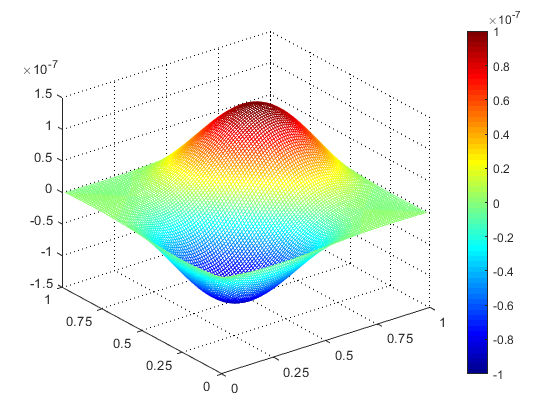
\includegraphics[width=0.7\linewidth]{fig/pscompact}
		\caption{紧致差分格式的DST快速算法绝对误差曲面}
	\end{figure}
	紧致差分格式的DST算法是非常强大的,相对于快速DST算法,紧致差分格式的DST算法精度更高,并且算法更为快速。
	
	\subsection{迭代求解法}
	令$s(x,y)=-f(x,y)$,对$\Delta u (x,y)=s(x,y)$进行中心差分:
	$$
	\frac{u_{i+1, j}-2 u_{i, j}+u_{i-1, j}}{\Delta x^{2}}+\frac{u_{i, j+1}-2 u_{i, j}+u_{i, j-1}}{\Delta y^{2}}=s_{i, j}
	$$
	令$I=J$,则
	$$
	u_{i+1, j}+u_{i-1, j}+u_{i, j+1}+u_{i, j-1}-4 u_{i, j}=h^{2} s_{i, j}
	$$
	重排列得:
	$$
	u_{i, j}=\frac{1}{4}\left[u_{i+1, j}+u_{i-1, j}+u_{i, j+1}+u_{i, j-1}-h^{2} s_{i, j}\right]
	$$
	即
	$$
	\left[\begin{array}{cccccccccc}
		-4 & 1 & 0 & 0 & \cdots & 1 & 0 & \cdots & \cdots & \cdots \\
		1 & -4 & 1 & 0 & \cdots & 0 & 1 & \cdots & \cdots & \cdots \\
		0 & 1 & -4 & 1 & \cdots & \cdots & 0 & 1 & \cdots & \cdots \\
		\vdots & & & & & \\
		\vdots & & & & & \\
		0 & & & & \\
		\vdots & & & & \\
		1 & 0 & & & \\
		0 & 1 & & \\
		0 & 0 & 1 & & \\
		& & \cdots & & & \cdots & & 0 & 1 & -4\\
	\end{array}\right]
	\left[\begin{array}{c}
		u_{1,1} \\
		u_{2,1} \\
		u_{2,2} \\
		\vdots \\
		\vdots \\
		u_{I, J-1} \\
		u_{I, J}
	\end{array}\right]
	=h^2\left[\begin{array}{c}
		s_{1,1} \\
		s_{1,2} \\
		\vdots \\
		s_{1, j} \\
		s_{2,1} \\
		s_{2,2} \\
		\vdots \\
		\vdots \\
		s_{I, J-1} \\
		s_{I, J}
	\end{array}\right]
	$$

	此方程式可以使用Jacobi迭代法和G-S迭代法求解,在判断收敛条件时,若相邻两次迭代的$U$向量距离的F范数小于$10^-4$,则判定为收敛。同样选择$N=100,n=1$,数值实验结果如下:
	\begin{figure}[H]
		\centering
		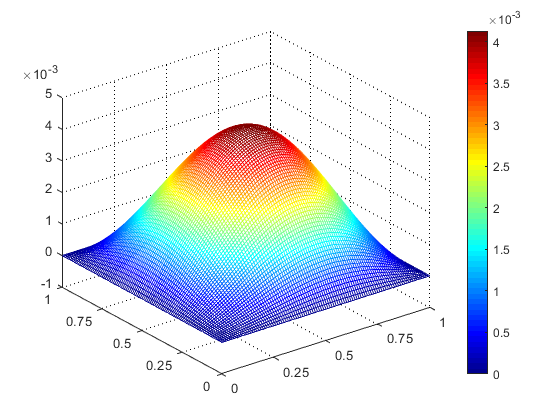
\includegraphics[width=0.7\linewidth]{fig/psjacobi}
		\caption{Jacobi迭代法的误差曲面}
	\end{figure}
	\begin{figure}[H]
		\centering
		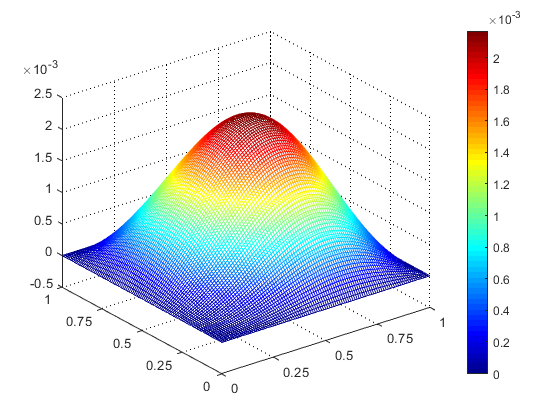
\includegraphics[width=0.7\linewidth]{fig/psgs}
		\caption{G-S迭代法的误差曲面}
	\end{figure}
	相对于快速DST算法和紧致差分格式的快速DST算法,Jacobi迭代法和G-S迭代法显得非常低效,误差更高,并且求解容易不稳定(一部分受限于MATLAB的循环性能)。
	
	\newpage
	\section{双曲线形的偏微分方程求解}
	取$a=1,2,h=0.1,\tau = 0.08$,求解一阶双曲方程:
	$$\left\{\begin{array}{l}u_{t}+a u_{x}=0 \\ u(0, x)=f(x)=\left\{\begin{array}{ll}1 & x \leq 0 \\ 0 & x>0\end{array}\right.\end{array}\right.$$
	
	方程的真实解为$u(x,t)=f(x-at)$,那么当$t=4$时,
	$$
	u(x, 4)=\left\{\begin{array}{ll}
		0, & x>4 a \\
		1, & x \leq 4 a
	\end{array}\right.
	$$
	
	求解分别采用空间向后的迎风格式(Upwind scheme)
	$$
	u_{j}^{n+1}=u_{j}^{n}-a \lambda\left(u_{j}^{n}-u_{j-1}^{n}\right)
	$$
	
	Lax-Friedrichs格式:
	$$
	u_{j}^{n+1}=\frac{1}{2}\left(u_{j+1}^{n}+u_{j-1}^{n}\right)-\frac{1}{2} a \lambda\left(u_{j+1}^{n}-u_{j-1}^{n}\right)
	$$
	
	Lax-Wendroff格式:
	$$
	u_{j}^{n+1}=u_{j}^{n}-\frac{1}{2} a \lambda\left(u_{j+1}^{n}-u_{j-1}^{n}\right)+\frac{1}{2} a^{2} \lambda^{2}\left(u_{j+1}^{n}-2 u_{j}^{n}+u_{j-1}^{n}\right)
	$$
	
	\subsection{迎风格式}
	迎风格式的基本思想是:在双曲型方程中关于空间偏导数用在特征线方向一侧的单边差商来代替,对应公式为:
	$$
	u_{j}^{n+1}=u_{j}^{n}-a \lambda\left(u_{j}^{n}-u_{j-1}^{n}\right)
	$$
	
	容易求出其在时间空间方向上均为一阶精度,即$L_h u (x,t)=\mathbb{O}(\tau + h)$,迎风格式的节点分布如下图:
	\begin{figure}[H]
		\centering
		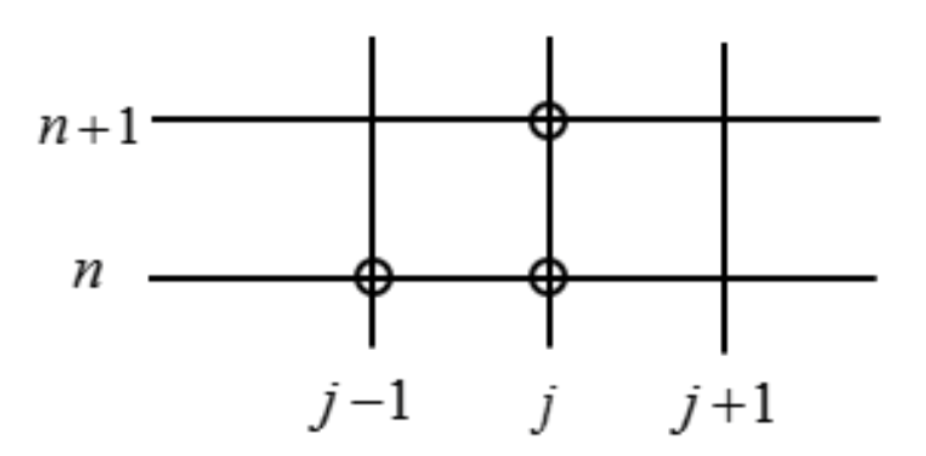
\includegraphics[width=0.7\linewidth]{fig/fig2}
		\caption{迎风格式的节点分布}
	\end{figure}

	使用傅里叶方法分析迎风格式的稳定性,令$u_{j}^{n}=v^{n} e^{i k j h}$,容易求出迎风格式的增长因子为:
	$$
	G(\tau, k)=1-a \lambda(1-\cos k h)-a \lambda i \sin k h
	$$
	因此
	$$
	|G(\tau, k)|^{2}=1-4 a \lambda(1-a \lambda) \sin ^{2} \frac{k h}{2}
	$$
	
	如果$a\lambda \le 1$ ,则有$|G(\tau, k)|^2 \le 1$,即Von-Neumannn条件满足。所以迎风格式在$a \lambda \le 1$时稳定。
	
	\subsection{Lax-Friedrichs格式}
	在空间方向上使用中心差分,可以得到逼近对流方程的一个中心差分格式:
	$$
	\frac{u_{j}^{n+1}-u_{j}^{n}}{\tau}+a \frac{u_{j+1}^{n}-u_{j-1}^{n}}{2 h}=0
	$$
	
	其截断误差为$\mathbb{O}(\tau + h^2)$,但其是绝对不稳定的差分格式。
	
	1954年,Lax和Friedrichs为克服上述格式的不稳定性,用$\frac{1}{2}\left(u_{j+1}^{n}+u_{j-1}^{n}\right)$代替其中的$u_j^n$,得到Lax-Friedrichs格式:
	$$
	\frac{u_{j}^{n+1}-\frac{1}{2}\left(u_{j+1}^{n}+u_{j-1}^{n}\right)}{\tau}+a \frac{u_{j+1}^{n}-u_{j-1}^{n}}{2 h}=0
	$$
	或写成
	$$
	u_{j}^{n+1}=\frac{1}{2}\left(u_{j+1}^{n}+u_{j-1}^{n}\right)-\frac{1}{2} a \lambda\left(u_{j+1}^{n}-u_{j-1}^{n}\right)
	$$
	
	Lax-Friedrichs格式的截断误差是$\mathbb{O}(\tau + h^2)+\mathbb{O}(\frac{h^2}{\tau})$。由于在双曲型方程的差分格式计算中,一般取网格比$\lambda = \frac{\tau}{h} = const$,所以Lax-Friedrichs格式是一阶精度的差分格式。Lax-Friedrichs格式的节点分布如下图:
	\begin{figure}[H]
		\centering
		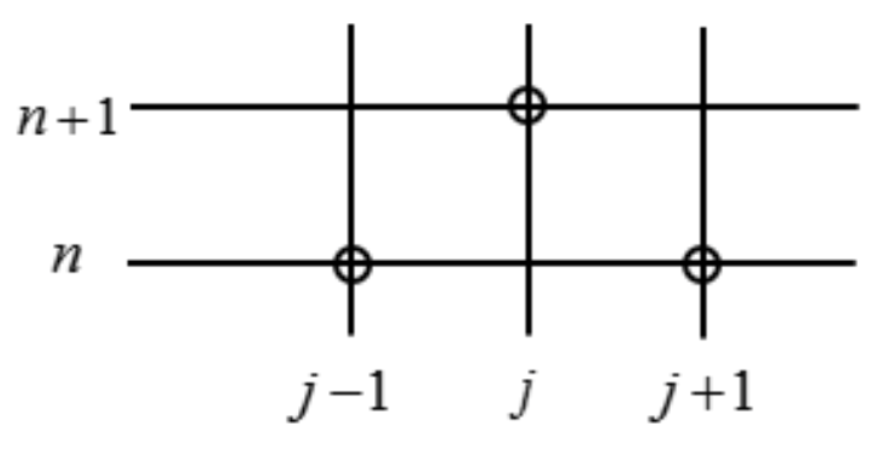
\includegraphics[width=0.7\linewidth]{fig/fig3}
		\caption{Lax-Friedrichs格式节点分布}
	\end{figure}
	
	使用傅里叶方法分析Lax-Friedrichs格式的稳定性,令$u_j = v^n e^{ikjh}$,容易求出Lax-Friedrichs格式的增长因子为:
	$$
	G(\tau, k)=\cos k h-i a \lambda \sin k h
	$$
	所以:
	$$
	|G(\tau, k)|^{2}=1-\left(1-a^{2} \lambda^{2}\right) \sin ^{2} k h
	$$
	
	当$|\alpha|\lambda \le 1$时有$|G(\tau , k)|^2 \le 1$,即Von-Neumann条件满足。
	
	所以Lax-Friedrichs格式在$|\alpha|\lambda \le 1$时稳定。
	
	\subsection{Lax-Wendroff格式}
	前面讨论的迎风格式和Lax-Friedrichs格式是一阶精度的差分格式。1960年Lax和Wendroff构造出一个二阶精度的二层格式,这个差分格式在实际计算中得到了充分的重视。
	
	设$u(t,x)$是微分方程的光滑解,将$u(x_j,t_{n+1})$在点$(x_j,t_n)$处做Taylor展开
	$$
	u\left(x_{j}, x_{n+1}\right)=u\left(x_{j}, t_{n}\right)+\tau\left[\frac{\partial u}{\partial t}\right]_{j}^{n}+\frac{\tau^{2}}{2}\left[\frac{\partial^{2} u}{\partial t^{2}}\right]_{j}^{n}+O\left(\tau^{3}\right)
	$$
	一阶双曲方程有:
	$$
	\begin{array}{c}
		\frac{\partial u}{\partial t}=-a \frac{\partial u}{\partial x} \\
		\frac{\partial^{2} u}{\partial t^{2}}=\frac{\partial}{\partial t}\left(-a \frac{\partial u}{\partial x}\right)=a^{2} \frac{\partial^{2} u}{\partial x^{2}}
	\end{array}
	$$
	因此有:
	$$
	u\left(x_{j}, x_{n+1}\right)=u\left(x_{j}, t_{n}\right)-a \tau\left[\frac{\partial u}{\partial x}\right]_{j}^{n}+\frac{a^{2} \tau^{2}}{2}\left[\frac{\partial^{2} u}{\partial x^{2}}\right]_{j}^{n}+O\left(\tau^{3}\right)
	$$
	用中心差商逼近上式中的导数项,有
	$$
	\begin{array}{l}
		{\left[\frac{\partial u}{\partial x}\right]_{j}^{n}=\frac{1}{2 h}\left[u\left(x_{j+1}, t_{n}\right)-u\left(x_{j-1}, t_{n}\right)\right]+O\left(h^{2}\right)} \\
		{\left[\frac{\partial^{2} u}{\partial x^{2}}\right]_{j}^{n}=\frac{1}{h^{2}}\left[u\left(x_{j+1}, t_{n}\right)-2 u\left(x_{j}, t_{n}\right)+u\left(x_{j-1}, t_{n}\right)\right]+O\left(h^{2}\right)}
	\end{array}
	$$
	得到
	$$
	\begin{aligned}
		u\left(x_{j}, x_{n+1}\right)=& u\left(x_{j}, t_{n}\right)-\frac{a \tau}{2 h}\left[u\left(x_{j+1}, t_{n}\right)-u\left(x_{j-1}, t_{n}\right)\right]+O\left(\tau h^{2}\right) \\
		&+\frac{a^{2}}{2} \frac{\tau^{2}}{h^{2}}\left[u\left(x_{j+1}, t_{n}\right)-2 u\left(x_{j}, t_{n}\right)+u\left(x_{j-1}, t_{n}\right)\right] \\
		&+O\left(\tau^{2} h^{2}\right)+O\left(\tau^{3}\right)
	\end{aligned}
	$$
	略去高阶项后得到Lax-Wendroff格式:
	$$
	u_{j}^{n+1}=u_{j}^{n}-\frac{a \tau}{2 h}\left(u_{j+1}^{n}-u_{j-1}^{n}\right)+\frac{a^{2}}{2} \frac{\tau^{2}}{h^{2}}\left(u_{j+1}^{n}-2 u_{j}^{n}+u_{j-1}^{n}\right)
	$$
	
	Lax-Wendroff格式的节点分布如下图:
	\begin{figure}[H]
		\centering
		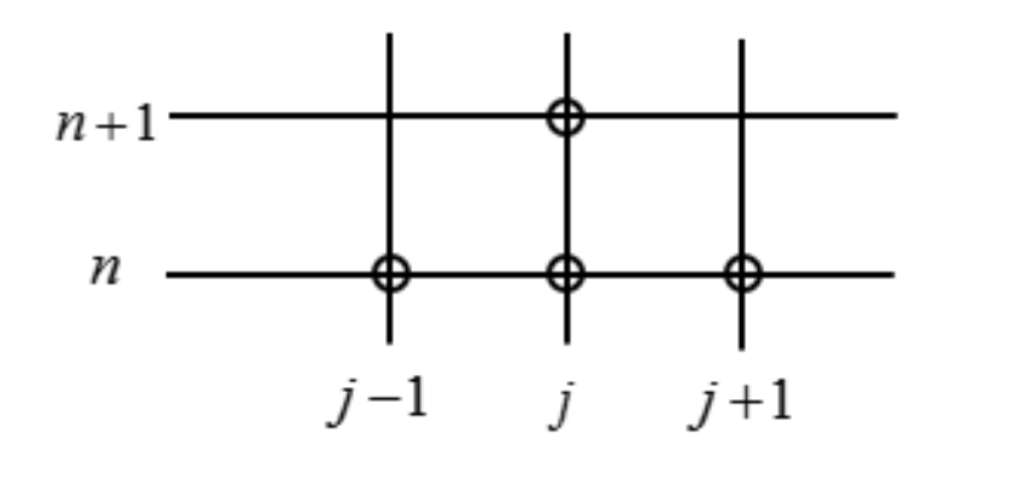
\includegraphics[width=0.7\linewidth]{fig/fig8}
		\caption{Lax-Wendroff格式节点分布}
	\end{figure}

	其增长因子为
	$$
	\begin{array}{l}
		G(\tau, k)=1-2 a^{2} \lambda^{2} \sin ^{2} \frac{k h}{2}-i a \lambda \sin k h \\
		|G(\tau, k)|^{2}=1-4 a^{2} \lambda^{2}\left(1-a^{2} \lambda^{2}\right) \sin ^{4} \frac{k h}{2}
	\end{array}
	$$
	当$|a|\lambda \le 1$时有$|G(\tau , k)|^2 \le 1$,即Von-Neumann条件满足。所以Lax-Wendroff格式在$|a|\lambda \le 1$时稳定。
	
	\subsection{实验结果及分析}
	当$a=1$时,三种差分格式的计算结果如图:
	\begin{figure}[H]
		\centering
		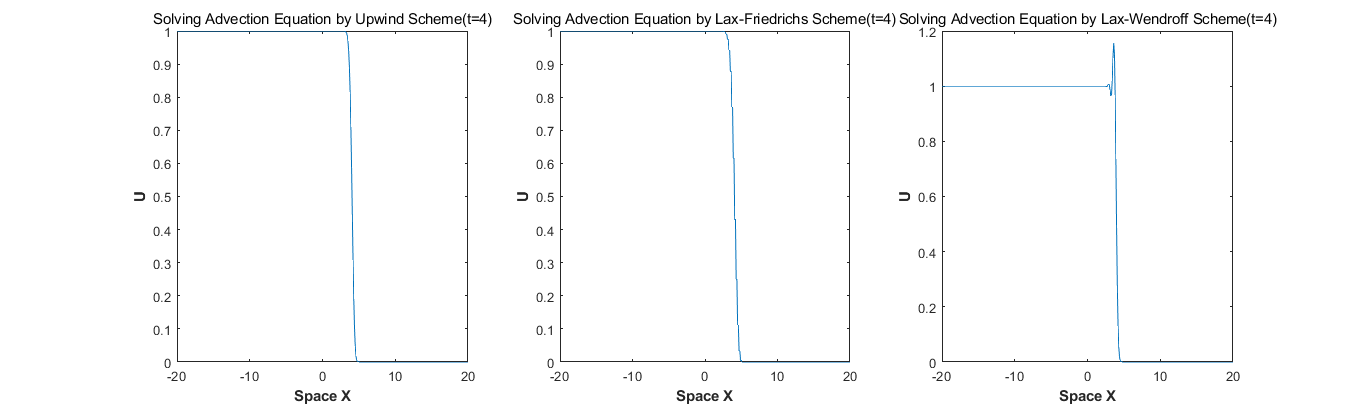
\includegraphics[width=\linewidth]{fig/fig4}
		\caption{迎风格式,Lax-Friedrichs格式,Lax-Wendroff格式计算结果时空分布(a=1)}
	\end{figure}

	其中$t=4$时计算结果的空间分布如下:
	\begin{figure}[H]
		\centering
		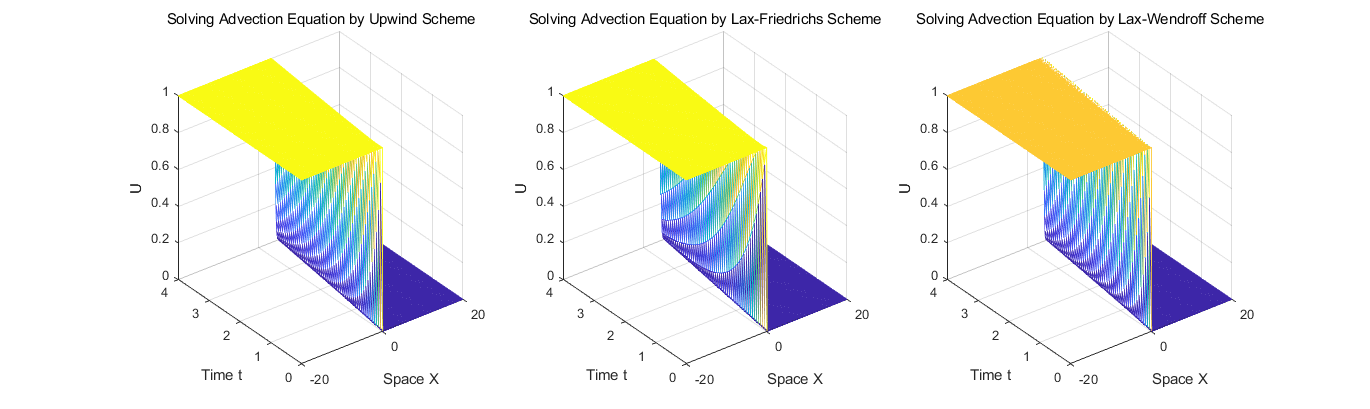
\includegraphics[width=\linewidth]{fig/fig5}
		\caption{迎风格式,Lax-Friedrichs格式,Lax-Wendroff格式计算结果$t=4$时刻空间分布(a=1)}
	\end{figure}

	当$a=2$时,三种差分格式的计算结果如图:
	\begin{figure}[H]
		\centering
		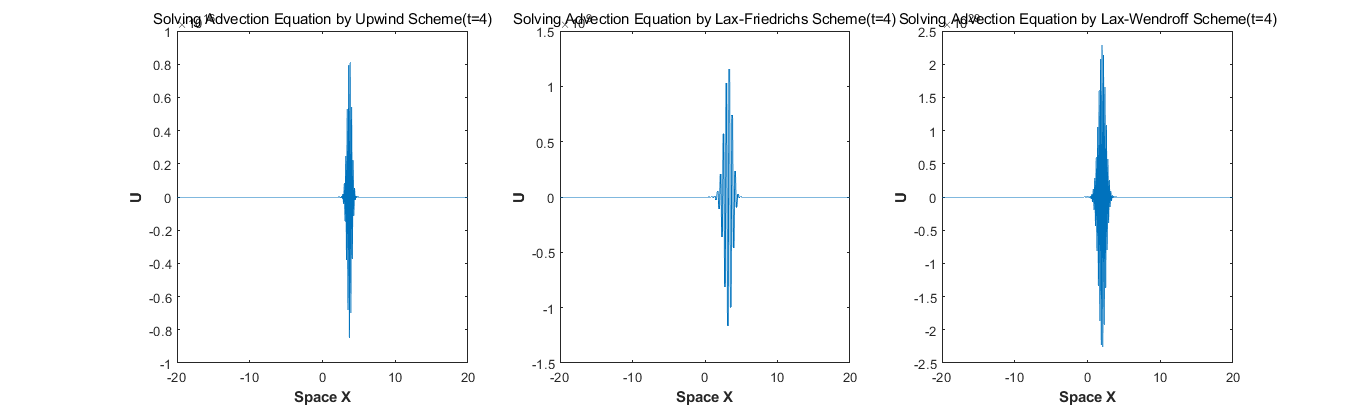
\includegraphics[width=\linewidth]{fig/fig6}
		\caption{迎风格式,Lax-Friedrichs格式,Lax-Wendroff格式计算结果时空分布(a=2)}
	\end{figure}
	
	其中$t=4$时计算结果的空间分布如下:
	\begin{figure}[H]
		\centering
		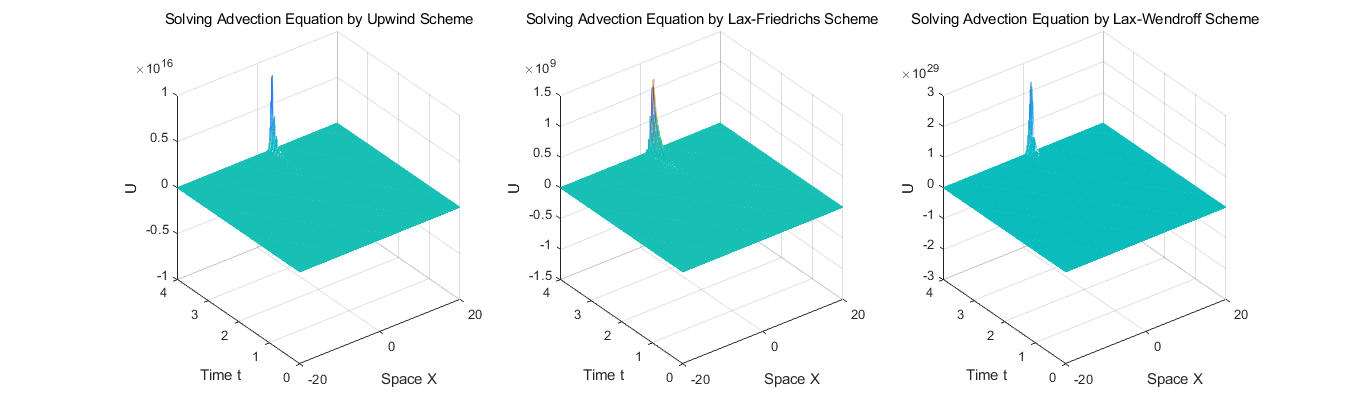
\includegraphics[width=\linewidth]{fig/fig7}
		\caption{迎风格式,Lax-Friedrichs格式,Lax-Wendroff格式计算结果$t=4$时刻空间分布(a=2)}
	\end{figure}

	由于网格比$\lambda = \frac{\tau}{h} = 0.8$,在$a=1$时,$|a|\lambda \le 1$,三种差分格式均可得到稳定计算结果。在$a=2$时,$|a|\lambda > 1$,三种差分格式不稳定,图中可以明显观察到这一结果。
	
	比较$a=1$时间断点处的计算结果,可以看出迎风格式、Lax-Friedrichs格式在间断点处的计算结果仍然较好,而Lax-Wendroff格式的计算结果在间断点处出现了波动。其原因在于Lax-Wendroff格式除了依赖于$u_{j-1}^n,u_j^n$外,还依赖于$u_{j+1}^n$。而根据对流方程的物理意义,在$a>0$时,其在$u(x_0,t_0 + \tau)$处的值只依赖于$u(x,t_0),x<x_0$处的值。该方程的初始条件在$x=0$处间断,即:
	$$
	u(0, x)=f(x)=\left\{\begin{array}{ll}
		1, & x \leq 0 \\
		0, & x>0
	\end{array}\right.
	$$
	
	在使用迎风格式、Lax-Friedrichs格式计算时,空间方向从左到右依次计算,计算$x=0$处的结果时,不会受到间断点后的结果影响。而使用Lax-Wendroff格式计算时,由于使用了$u_{j+1}^n$时的值,在计算$x=0$的结果的时候,会受到间断点后的影响,所以其数值解在间断点后会有波动现象出现。
	
	
	
	
	\newpage
	\section{抛物线形的偏微分方程求解}
	考虑二维扩散方程:
	$$
	\left\{\begin{array}{l}
		u_t = \frac{\partial ^2 u}{\partial x^2} + \frac{\partial ^ 2 u}{\partial y ^ 2} = U_{xx}  + u_{yy} \quad \text { in } \Omega \\
		u(x,y,0) = \sin(\pi x + \pi y)
		u=0 \text { on } \partial \Omega
	\end{array}\right.
	$$
	
	式中$\Omega = (0,1) \times (0,1)$。
	
	方程的真实解为:
	$$
	u(x,y,t) = \exp (-t) \sin(\pi x) \cos(\pi y)
	$$
	
	取空间步长$h = l/M$,时间步长$\tau > 0$,作两族平行于坐标轴的网线:$x = x_j = jh, y = y_k = kh,k=0,1,\cdots,M$,将区域$0 ]e x,y \le 1$分割成$M^2$个小矩形。ADI方法(交替方向隐格式)是将第$n$层到第$n+1$层计算分成两步:先由第$n$层到第$n+\frac{1}{2}$层,对$u_{xx}$用向后差分逼近,对$u_{yy}$用向前差分逼近,然后由第$n+\frac{1}{2}$到第$n+1$层,对$u_{xx}$用向前差分逼近,对$u_{yy}$用向后差分逼近,于是得到ADI格式:
	$$
	\begin{array}{l}
		\frac{u_{i j}^{n+1 / 2}-u_{i j}^{n}}{\Delta t / 2}=\left(\delta_{x}^{2} u_{i j}^{n+1 / 2}+\delta_{y}^{2} u_{i j}^{n}\right) \\
		\frac{u_{i j}^{n+1}-u_{i j}^{n+1 / 2}}{\Delta t / 2}=\left(\delta_{x}^{2} u_{i j}^{n+1 / 2}+\delta_{y}^{2} u_{i j}^{n+1}\right)
	\end{array}
	$$
	
	这样,该方程系统涉及一个对称阵和一个三角矩阵,可以用三对角阵的求解算法进行计算。该方法绝对稳定,因此受到人们的普遍注意。
	
	\subsection{实验结果}
	当$t=0.01$时,ADI方法的计算结果如图:
	\begin{figure}[H]
		\centering
		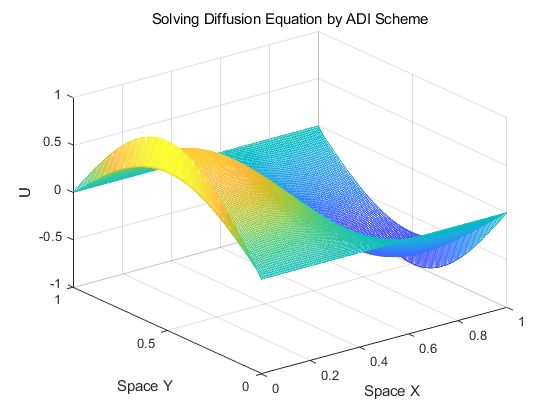
\includegraphics[width=0.7\linewidth]{fig/adi}
		\caption{ADI格式计算结果}
	\end{figure}
	
	扩散方程的真实解结果为:
	\begin{figure}[H]
		\centering
		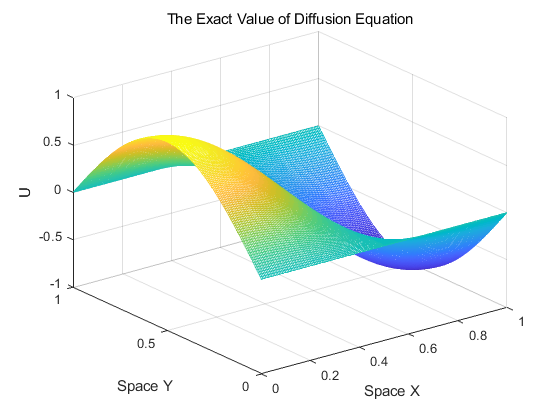
\includegraphics[width=0.7\linewidth]{fig/exact}
		\caption{扩散方程真实解}
	\end{figure}
	
	误差为:
	\begin{figure}[H]
		\centering
		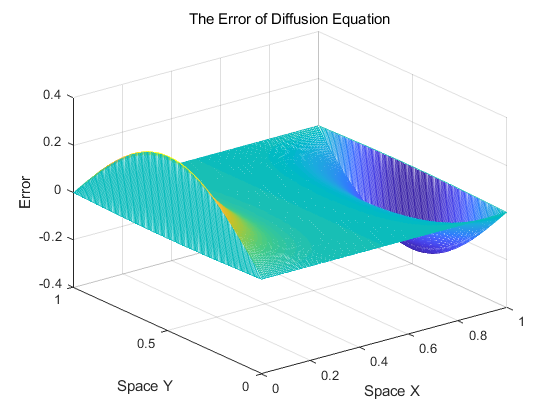
\includegraphics[width=0.7\linewidth]{fig/err}
		\caption{ADI格式误差}
	\end{figure}
	
\end{document}